

\section{Introduction}
Recall from \cref{sec:howtotransport} that STImulated Raman Adiabatic Passage (STIRAP) is a state transfer protocol that acts on a three-state system. Labeling the states as $\{ \ket{j} \}_{j=1}^3$, the protocol maps the state $\ket{1}$ to state $\ket{3}$ without requiring any direct interaction between $\ket{1}$ and $\ket{3}$. Rather, it couples these states to some intermediate state $\ket{2}$ by two tuned laser pulses \cite{Gaubatz1990}. A distinguishing feature is that state $\ket{2}$ is minimally populated, making the evolution largely insensitive to decoherence due to the intermediate state \cite{Vitanov2017}. The protocol is now widely adopted in fields where accurate control of quantum states is vital, such as high precision measurement \cite{Kasevich2002,Kotru2015}, studies of atoms and molecules \cite{Kral2007,Stellmer2012,Petrosyan2015,Moses2017,Ciamei2017}, and quantum information processing \cite{Pachos2002,Troiani2003,Paspalakis2004,Timoney2011,Koh2013}. A recent review of results and applications can be found in Ref. \cite{Vitanov2017}. 

A mathematically equivalent protocol can be used to spatially displace quantum amplitudes. In 2004, two independent works proposed state transfer of quantum particles over linear chains, by tuning the hopping strengths instead of laser fields: Ref. \cite{Eckert2004} considered neutral atoms in optical lattices, whilst Ref. \cite{Greentree2004} addressed electrons tunneling between quantum dots. The latter introduced the name Coherent Tunneling by Adiabatic Passage (CTAP), which we will also use to denote spatial transfer. Apart from particle tunneling, the same model applies to ferromagnetic spins under XX interaction \cite{Ohshima2007}, where a single spin excitation can be adiabatically transferred. 

%
%

With the advent of quantum information processing, accurate control and high-fidelity qubit transport in increasingly large systems have become an important scientific challenge \cite{DiVincenzo2000,Preskill2018}.  As we argue in \cref{sec:transfergeneralgraphs}, the majority of scientific attention focused on transfer over linear chains \cite{Vitanov2017, Menchon-Enrich2016}, whilst little is known about adiabatic transfer in more general systems. Already in the 90s, STIRAP was generalized to linear chains of odd length $N$, allowing transfer between the endpoints of the chain \cite{Malinovsky1997}. More recent work includes Refs. \cite{Bradly2012,Longhi2014}, which consider square and triangular grids, and Ref. \cite{Greentree2006}, which addresses multiple parties dangling on a line, each of whom could send or receive the quantum state. Other works, such as Refs. \cite{Chen2013,Batey2015} describe a variation where the chain splits into multiple paths or branched endpoints. These protocols are shown to work by a clever mapping back to the original protocol on the chain.  

%

We aim to find more general configurations that allow a similar transfer protocol, by describing a system's interactions in the language of graphs (\cref{sec:graphs}): the vertices represent basis states and edges represent interactions. We look at bipartite graphs, where the basis states can be separated into two sets $V_1$ and $V_2$, such that each state interacts only with states outside its own set. 
If the two sets differ in size by one, then amplitude transfer between states in the bigger set may be possible. We can guarantee successful transfer when certain graph properties are satisfied, as made precise in \cref{thm:transfer}. 

Interestingly, our approach naturally provides a means to transfer amplitude to one out of multiple potential receivers, generalizing Ref. \cite{Greentree2006}. We find that the final receiver need not yet be known when starting the protocol, which could be an advantage in quantum information processing. 

These results advance the fields of STIRAP and spatial transfer in two ways. Firstly, they open the way to practical adiabatic passage in more general systems. Secondly, they shed light on possible perturbations in conventional STIRAP and their effect: we find that many perturbations, as long as they satisfy our assumptions, do not cause a qualitatively different effect on the state's evolution during the protocol. 

Our treatment of bipartite graphs is reminiscent of the celebrated Morris-Shore (MS) transformation \cite{Morris1983}. The transformation finds a unitary map $A$ on the part $V_1$ and a unitary map $B$ on part $V_2$, such that the system decomposes into a set of decoupled two-level systems, and a set of uncoupled states. Similar to the setting of MS, we focus on the uncoupled states, which are called dark states. Our contribution is distinct from work related to MS transformations, due to the focus on adiabatic transfer techniques, in which the MS transformation would continuously change in time. Therefore, it is not immediately clear how MS could guarantee that our adiabatic state remains nondegenerate, and we choose to resort to other techniques. 

 
This chapter is organized as follows. In \cref{sec:conventional}, we review the conventional STIRAP and CTAP protocol, after which we present our main result on more general graphs in \cref{sec:generalizing}. We then discuss the applicability in real-world systems in \cref{sec:CTAPapplications}, and methods to obtain graphs that satisfy our assumptions in \cref{sec:viablegraphs}. We numerically test the scaling of the adiabatic gap in various graphs, and the fidelity of our protocol, in \cref{sec:CTAPnumerics}, and finish with a conclusion in \cref{sec:conclusion}.


\section{Conventional STIRAP}
\label{sec:conventional}

\begin{figure}[t]
\centering
\def\svgwidth{.7\linewidth}
\input{img/intro_stirap_basics_3.pdf_tex}
\caption{The conventional STIRAP/CTAP protocol on a three-site $\Lambda$ system. \textbf{(a)} The energy diagram of the three states, coupled by the Stokes (S) and Pump (P) lasers, also represented as a graph in \textbf{(b)}. \textbf{(c)} Stacked plot showing the laser amplitudes, state amplitudes, and energies (eigenvalues $\lambda$) as a function of time, in arbitrary units. Stages I and III involve turning the couplings on/off, whereas stage II constitutes the relevant adiabatic driving part which transfers amplitude from state $\ket{1}$ to $\ket{3}$ as amplitudes $\Omega_S$ and $\Omega_P$ are slowly adjusted relative to each other. }
\label{fig:stirap}
\end{figure}


The conventional STIRAP protocol (\cref{fig:stirap}) deals with a three-dimensional quantum system, consisting of eigenstates $\{\ket{j}\}_{j=1}^3$ of some background Hamiltonian. To transfer amplitude from $\ket{1}$ to $\ket{3}$, a sequence of two laser pulses is applied: the Stokes pulse coupling $\ket{2} \leftrightarrow \ket{3}$, and the Pump pulse coupling $\ket{1} \leftrightarrow \ket{2}$. Throughout this section, we consider only the interaction picture and assume the rotating wave approximation to hold. The system's Hamiltonian then becomes
\begin{align}
H = \begin{pmatrix}
0 & \Omega_P(t) & 0 \\
\Omega_P(t) & \varepsilon & \Omega_S(t) \\
0 & \Omega_S(t) & 0
\end{pmatrix}.
\label{eq:Hstirap}
\end{align}
Here, $\Omega_{S/P}$ denotes the Rabi frequency (amplitude) of the Stokes and Pump lasers, respectively, and $\varepsilon$ absorbs the off-resonances, assuming both are equal in size. 
One can check that one instantaneous eigenstate of $H$ is the zero energy `dark state' $\ket{z}$ given by 
\begin{align*}
\ket{z(t)} = \frac{1}{\mathcal{N}} \begin{pmatrix}
\Omega_P^{-1}(t) \\ 0 \\ -\Omega^{-1}_S(t)
\end{pmatrix},
\end{align*}
where $\mathcal{N}$ denotes the normalization. The dark state $\ket{z}$ has precisely the property that it transitions from $\ket{1}$ to $\ket{3}$ as $\Omega_S$ is gradually diminished while $\Omega_P$ is increased. 
Note the counter-intuitive order of the pulses, as indicated in \cref{fig:stirap}. 
A key property of STIRAP is that the excited state $\ket{2}$ is never populated during this process, hence the protocol is independent of decoherence due to emission from this state. 
Thanks to this, and the inherent stability of adiabatic methods \cite{Childs2001}, the protocol is relatively stable to experimental imperfections, and is broadly adopted in practice \cite{Vitanov2017}. 

The setting where quantum particles can tunnel between three adjacent sites is mathematically equivalent to \cref{eq:Hstirap}, where the parameters $\Omega$ now take the role of tunneling amplitudes. The same protocol can then be applied, leading to transfer of the particle wavefunction, as is the case in CTAP.




\section{Generalizing STIRAP}
\label{sec:generalizing}
We observe that a key property of STIRAP and CTAP is the existence of a unique zero-energy eigenstate at all times (guaranteeing adiabatic transfer), and that this state is localizable by lowering couplings incident to a particular site. This leads us to our main question: which other physical configurations pertain \emph{precisely} one zero eigenvector, even when uncoupling a certain site?

We capture the more general configurations in the language of \emph{weighted graphs} $G = (V,E,w)$. Here, the collection of vertices $V = \{v_j \}_{j=1}^{\dim(\mathcal{V})}$ corresponds to a set of basis states $\{ \ket{v_j} \}_{j=1}^{\dim(\mathcal{V})}$ of Hilbert space $\mathcal{V}$. %
Two vertices $v,u \in V$ are connected by an edge $(u,v) \in E$ if and only if an interaction that couples states $\ket{u}$ and $\ket{v}$ can be applied. The weights $w : E \rightarrow \mathbb{C}$ assign a complex amplitude to each of the interactions. Weights evaluated on non-existent edges are zero: $w_{uv} = 0  $ for all $(u,v) \not \in E$.  
In the context of CTAP, the vertices should be interpreted as sites for the particle, and the edges indicate possible tunneling of the particle. In the context of STIRAP, vertices are energy levels, and edges are possible couplings by laser fields.

The \emph{adjacency matrix} $A_G$ of a graph is then defined as the matrix of weights, with matrix elements $(A_G)_{uv} = w_{uv}$. We impose hermiticity through $w_{uv} = w^*_{vu}$.
For computational simplicity, we take the adjacency matrix to be constant (we consider it as a background), and define the \emph{control Hamiltonian} $H_G$ for a given graph $G$ by
\begin{align*}
H_G(t) = \sum_{u,v \in V} f_{uv}(t) w_{uv} \ket{u} \bra{v}\,, && f_{uv}(t) = f^*_{vu}(t) \,.
\end{align*}
In this definition of the control Hamiltonian, we assume arbitrary time-dependent control over each allowed interaction, by tuning the \emph{controls} $f_{uv}(t)$. %

The graph $G$ from which $H_G$ is derived will be called the \emph{interaction graph}, which restricts the allowed interactions in $H_G$. In the context of quickly oscillating laser fields, we obtain Hamiltonians $H$ that are effectively time-independent except for the envelopes given by the functions $f_{uv}(t)$. The Hamiltonians we consider thus correspond to the interaction picture, in which quickly oscillating fields have either been absorbed into the on-site energies in the rotating frame, or where off-resonant fields are neglected by the rotating wave approximation. 


Thanks to the mapping to graphs, we can use various notions from graph theory. We denote with $G-v$ the graph $G$ in which the vertex $v$ and all the edges incident to $v$ are removed. A \emph{bipartite graph} has a vertex set $V$ which can be separated into two independent subsets $V_1, V_2$ such that each edge $(u,v) \in E$ must run \emph{between} $V_1$ and $V_2$ (that is, $u \in V_1$ and $v \in V_2$ or vice-versa). In the following, we will encounter a certain variation on bipartite graphs:
%
\begin{definition}
A \emph{semi-bipartite graph with parts $V_1$ and $V_2$} \cite{Xu2010,Al-Kofahi2009} is a bipartite graph in which edges within $V_2$ are allowed (including self-loops), but edges within $V_1$ are still prohibited. For example, the graph in \cref{fig:stirap} is semi-bipartite with $V_1 = \{ \ket{1}, \ket{3} \}$, but not bipartite unless the self-loop (the off-resonance of $\ket{2}$) is removed.
\end{definition}
%
Note that for a connected bipartite graph, the decomposition $ V = V_1 \sqcup V_2$ is determined uniquely (up to interchanging $V_1$ and $V_2$), while this is almost never the case for semi-bipartite graphs: any vertex in $ V_1$ may be moved to $V_2$. Hence, the decomposition is an essential part of the data. However, for our results, we want to take $|V_1| = |V_2|+1$, which means we cannot easily move points from $V_1$ to $V_2$.

We let $\mathcal{V}$ denote the vector space spanned by the states $\ket{v}$ corresponding to the vertices $v$ in $V$. Likewise, we use $\mathcal{V}_1, \mathcal{V}_2$ to denote the subspaces corresponding to subsets $V_1$, $V_2$. We order the basis of $\mathcal{V}$ by first stating the elements of $\mathcal{V}_1$ and then the elements of $\mathcal{V}_2$. In this basis, the interaction graph has the form
\begin{align}
A_G=\begin{pmatrix} 0 & B \\ B^T & C \end{pmatrix}\,,
\label{eq:bipgraph}
\end{align}
where $B$ is a matrix of size $|V_1| \times |V_2|$ and $C$ has size $|V_2| \times |V_2|$. We will mostly use this form of $A_G$ throughout this chapter. 


\begin{definition}
We use \emph{commensurate couplings} to denote the choice of couplings $f_{uv}(t)$ such that 
\begin{align*}
f_{v u}(t) &= f_v(t) && \forall\, u \in V_2,v\in V_1 \,;\\
f_{v u}(t) &= 1  && \forall\,  u,v \in V_2\,.
\end{align*}
In other words, for each vertex $v \in V_1$, the incident couplings are changed proportionally, whereas all couplings within $V_2$ to be equal to one.
\end{definition}

Note that the statement about commensurate couplings covers all couplings in a semi-bipartite graph. In such cases, with the interaction graph given in the form of \cref{eq:bipgraph}, we may write
\begin{equation}\label{Hamiltonianasconjugateadjacency}
H_G(t) = F(t) A_G F^*(t)\,,
\end{equation} 
where $F(t) = \mathop{\textup{diag}} (f_1(t), \dotsc , f_{|V_1|}(t), 1, \dotsc 1)$. 


We are now ready to state our main result. Consider a set of parties (vertices) $P\subseteq V_1$ located on a graph, who want to send a quantum state to each other. This turns out to be possible with a control Hamiltonian $H_G$, under certain graph restrictions, as made precise below. 

\begin{theorem}
\label{thm:transfer}
Let $G = (V,E,w)$ be a connected, weighted, semi-bipartite graph with parts $V_1$ and $V_2$. Let $P = \{p_j\}_{j=1}^k \subseteq V_1$. We assume that
\begin{itemize}
\item[1.] $|V_1| = |V_2| + 1$;
\item[2.] Either of the following:
\begin{itemize}
\item[2a.] For all $p_j$, $\det(A_{G-p_j}) \neq 0$;
\item[2b.] $A_G$ has a unique zero eigenvector, which has nonzero amplitude on each $p_j$.
\end{itemize}
\end{itemize}
Then, for any $a, b \in P$, the following choice of commensurate couplings are such that $H_G(t)$ adiabatically transfers amplitude from $a$ to $b$ in total time $T$:
\begin{equation}
\begin{split}
f_a(0) &= 0 \,; \\
f_b(T) &= 0 \,; \\
f_v(t) &\neq 0 \text{ for all $v \not \in P$;}\\
\text{No two }&\text{$f_v(t) $ may be zero simultaneously.}
\end{split}
\label{eqn:control_scheme} 
\end{equation}
\end{theorem}
%
Before we prove this theorem, we would like to analyse the statement first. The proof is given on \cpageref{prf:thmCTAP}, after \cref{Implicationatob}.

Firstly, note that $\det(A) \neq 0$ implies that $A$ does not have a zero eigenvalue. 

Moreover, the only couplings $f_{uv}$ that actually \emph{require} time-dependent control are those directly connected to sender and receiver; controlling any of the other couplings is optional. In fact, the control procedure can be performed locally and sequentially: it is possible to first only change the controls near $a$ and then only those near $b$. An example is the choice
\begin{equation*}
    f_v(t) = 
    \begin{cases}
        \min \{ 2t/T,1\} & v =a\,;\\
        \min \{1-2t/T,1\} & v=b\,;\\
        1 &\text{else}.
    \end{cases}
\end{equation*}
In particular, the receiver, $b$, can be chosen after the process has been initialized. 


%
%
%

The assumptions \emph{2a} and \emph{2b} are equivalent under the assumption of \emph{1}. More precisely, the following proposition holds.

\begin{proposition}\label{prop:2conditionsequiv}
Let $G = (V,E,w)$ be a weighted, semi-bipartite graph with parts $V_1$ and $V_2$, such that $ |V_1| = |V_2| + 1$, and let $ p \in V_1$. Then the following are equivalent:
\begin{itemize}
    \item[a.] $\det (A_{G-p}) \neq 0$;
    \item[b.] $A_G$ has a unique zero eigenvector, which has non-zero amplitude on $p$.
\end{itemize}
\end{proposition}
\begin{proof}
Let us first show that, thanks to $|V_1| = |V_2|+1$, there must exist a zero-energy eigenvector $\ket{z} = (z_1, 0) \in \mathcal{V}_1$ whose nonzero amplitudes $z_1$ are only located on sites in $V_1$. This holds because in the eigenvalue equation, using the form of \cref{eq:bipgraph},
\begin{align*}
\begin{pmatrix} 0 & B \\ B^T & C \end{pmatrix} \begin{pmatrix} z_1 \\ 0 \end{pmatrix}  = \begin{pmatrix} 0 \\ B^T z_1 \end{pmatrix} = 0\,,
\end{align*}
the system of equations $B^T z_1 = 0$ has $|V_1|$ variables and $|V_2|$ constraints, hence it must always have at least one non-trivial solution.

We start with the implication from \emph{a} to \emph{b}.
By the the previous argument, the rank of $ A_G $ can be at most $ |V|-1 $. However, as $\det (A_{G-p}) \neq 0$, the submatrix $A_{G-p}$ must be of maximal rank, which is also $ |V|-1$. As the rank of a submatrix gives a lower bound on the rank of a matrix, this shows that $ \rk A_G \geq |V|-1$. Therefore, there is a unique zero eigenvector.\par
Let this eigenvector be $v$, let its component at $p$ be $v_p$, and its components away from $p$ be $\tilde{v}$ (so $\tilde{v} $ is a vector with $|V|-1$ components). We can write $A_G $ as a block matrix
\begin{equation*}
  A_G = \begin{pmatrix} 0 & b_p \\ b_p^T & A_{G-p} \end{pmatrix} \,, 
\end{equation*}
where we wrote the component $p$ as the first component for simplicity. As $v$ is a zero eigenvector, we get
\begin{equation*}
    0 = A_G v = \begin{pmatrix} 0 & b_p \\ b_p^T & A_{G-p} \end{pmatrix} \begin{pmatrix} v_p \\ \tilde{v}\end{pmatrix} = \begin{pmatrix} b_p \tilde{v} \\ b^T_p v_p + A_{G-p} \tilde{v} \end{pmatrix}\,.
\end{equation*}
If now $ v_p =0$, then $ \tilde{v} \neq 0$, as an eigenvector cannot be zero, but then $A_{G-p}\tilde{v} \neq 0$, as $\det (A_{G-p}) \neq 0$. This is a contradiction, so we must have $ v_p \neq 0$.\par
Now we prove the implication from \emph{b} to \emph{a} by counterpositive. Hence we assume $\det (A_{G-p})=0$, and show that there exists a zero eigenvector of $A_G$ whose $p$-component is zero. Again, for notational simplicity, we write the component $p$ as the first component, so we have
\begin{equation*}
    A_{G} = \begin{pmatrix} 0 & B \\ B^T & C\end{pmatrix} = \begin{pmatrix} 0&0 & b_p \\ 0 & 0 & \tilde{B} \\ b_p^T & \tilde{B}^T & C \end{pmatrix}\,.
\end{equation*}
From this, we get
\begin{equation*}
    A_{G-p} =  \begin{pmatrix}  0 & \tilde{B} \\ \tilde{B}^T & C \end{pmatrix}\,,
\end{equation*}
where, crucially, the sizes of $ \tilde{B} $ and $C$ are equal by the assumption $ |V_1| = |V_2| + 1$. Hence,
\begin{equation*}
    \det (A_{G-p}) = \pm \det (\tilde{B} \tilde{B}^T ) = \pm \det (\tilde{B})^2\,.
\end{equation*}
Now, by assumption $ \det (A_{G-p}) =0$, so $ \det (\tilde{B}^T) = 0$. Therefore, there exists a zero eigenvector $u$ of $\tilde{B}^T$. If we define $v = (0, u, 0)$, then
\begin{equation*}
    A_{G} v = \begin{pmatrix} 0&0 & b_p \\ 0 & 0 & \tilde{B} \\ b_p^T & \tilde{B}^T & C \end{pmatrix} \begin{pmatrix}0 \\ u \\ 0 \end{pmatrix} = \begin{pmatrix} 0 \\ 0 \\ \tilde{B}^T u\end{pmatrix} =0\,,
\end{equation*}
so we have constructed a zero eigenvector of $A_G$ with zero amplitude on $p$, giving a contradiction.
\end{proof}

\begin{remark}\label{Implicationatob}
In fact, the implication from \emph{a} to \emph{b} goes through even in the case $G$ is not semi-bipartite; the proof does not use this assumption. However, for the other direction, it is essential.
\end{remark}



\begin{proof}[Proof of \cref{thm:transfer}]
\label{prf:thmCTAP}
By the first part of the proof of \cref{prop:2conditionsequiv}, there exists a zero-energy eigenvector $\ket{z}$ for any choice of controls.

Clearly, the couplings $f_{uv}(t)$ in \cref{eqn:control_scheme} are such that at times $0$ and $T$, the respective states $\ket{a}$ and $\ket{b}$ are zero-energy eigenstates. We will argue that, using the given control scheme, the zero-energy subspace is one-dimensional at all times. 

When all controls $f_{v}$ are equal to one, then $H_G = A_H$ and the zero-energy eigenstate $\ket{z}$ is unique, by assumption~\emph{2}. When the couplings change commensurately, as long as they remain non-zero, the eigenstate $\ket{z}$ changes as
\begin{align}
    \ket{z(t)} \propto F(t)^{-1} \ket{z},
    \label{eq:darkstate}
\end{align} %
as can be seen from \cref{Hamiltonianasconjugateadjacency}. Because $F$ is diagonal, $ \ket{z(t)}$ is still located on $V_1$. It is unique, because given any zero eigenvector $\ket{w} $ of $H_G(t)$, $F(t)\ket{w}$ is an eigenvector of $A_G$, hence must be equal, up to scaling, to $ \ket{z}$.

Special care has to be taken when reducing weights to zero. When reducing $f_p ~ (p \in P)$ towards zero, assumption~\emph{2a} guarantees that no zero eigenvectors occur on $G-p$, hence $\ket{p}$ must then be the unique zero eigenstate. %

This shows that any controls $f_v$ satisfying \cref{eqn:control_scheme} indeed pertain a unique zero-energy eigenstate, and provide the correct initial and final state at times $t=0$ and $t=T$. By the adiabatic theorem, a sufficiently high protocol time $T$ allows state transfer at arbitrary accuracy.
\end{proof}

The unique zero-eigenstate $\ket{z(t)}$ has many favorable stability properties. Its eigenvalue is \emph{exactly} $0$ throughout the whole protocol, independent of changes to $w_{uv}$, as long as the graph remains semi-bipartite. The constant energy makes the state's dynamical phase easy to track. Moreover, it has exactly $0$ amplitude on $\mathcal{V}_2$, which makes it insensitive to any decoherence on sites in $V_2$. The state $\ket{z}$ generalizes the `dark state' of conventional STIRAP and CTAP, inheriting important features that make these protocols attractive for practical purposes. 

One might be concerned that, when reducing all controls $f_{p_j v}$ incident to a certain party $p_j$ to zero, it is hard to maintain the commensurate ratios between the couplings. Luckily, it turns out that in such cases, commensurateness is not essential: the condition $\det(A_{G-p_j}) \neq 0$ guarantees that the zero eigenstate remains unique as long as all other sites remain commensurately coupled. This holds because the rank of $A_G$ must be at least that of $A_{G-p_j}$, which shows that for \emph{any} couplings between $p_j$ and the rest of the graph, there can be at most one zero-energy state. This freedom gives the protocol a convenient stability to imperfect controls.

 The time scale $T$ required by the protocol is determined by the gap in the spectrum around the zero eigenvalue, as opposed to the well-studied gap between the lowest and second lowest energy \cite{Brouwer2012}. To our best knowledge, little is known about the gap around zero, and characterizing its scaling is an interesting open problem. In \cref{sec:CTAPnumerics} we numerically study the scaling for certain example graphs. 







\section{Applications}
\label{sec:CTAPapplications}
Our main result requires a physical system to obey our conventions of control Hamiltonian $H_G$ for certain graphs $G$, with sufficiently flexible controls $f_{uv}$. Recall from \cref{sec:transfer_single_exc} that this applies to the case of \emph{single excitation hopping}, which describes the following example systems:
\begin{itemize}
\item Discrete energy levels coupled by (near-)resonant laser fields, like electronic levels in atoms or molecules, such as typically considered in STIRAP \cite{Vitanov2017}. The lasers can also be off-resonant, as long as each state in $V_2$ has all of its incident couplings at the same off-resonance. Either way, a transformation to the interaction picture, and assumption of the Rotating Wave Approximation are required. 
\item Systems where a quantum particle `hops' between coupled sites, such as electrons caught in quantum dots \cite{Greentree2004,Hensgens2017}, or atoms or atomic condensates trapped in optical potentials \cite{Eckert2004,Graefe2006,Bloch2012}. 
\item An XX model of interacting spins, of the form 
\begin{align*}
H_\text{XX} = \frac{1}{2} \sum_{uv \in E} w_{uv} \left( X_u X_v + Y_u Y_v \right) + h \sum_{u \in V} Z_u,
\end{align*}
where $\{X_u,Y_u,Z_u\}$ are the Pauli matrices acting on the site $u$, in the sector with a single spin excitation \cite{Ohshima2007}. 
\end{itemize}

The most interesting application might be in quantum information processing. As discussed in \cref{sec:transfer_single_exc}, quantum information can be transmitted whenever the states $\ket{j}$ represent the position of a quantum particle with internal degrees of freedom, as is the case with CTAP, or when a superposition between a shared vacuum and an excitation on a graph may be made. The latter applies to the XX model, where an initial state of the form
\begin{align*}
\ket{\psi(0)} = \alpha \ket{0}_a \ket{0\ldots 0} + \beta \ket{1}_a \ket{0 \ldots 0}
\end{align*}
can be initialized locally at site $a$. 

In the context of information transfer, care has to be taken with the additional phase that is picked up throughout the protocol.  As an example, in the XX model described above, the single-excitation subspace amplitude $\beta$ picks up a relative phase $\beta \rightarrow e^{- i h T} \beta$ relative to the vacuum amplitude $\alpha$. Moreover, the transfer protocol itself gives an additional phase to the transferred excitation, as previously observed by Ref. \cite{Greentree2006}. This becomes relevant when dealing with the XX model, or when transporting entangled particles or states. Owing to \cref{eq:darkstate}, as long as the controls $f_{uv}(t)$ remain real-valued, the additional phase acquired by the state when transferring from site $a$ to $b$ is equal to $\arg( z_a / z_b )$, where $z_a, z_b$ are elements of the zero-eigenvector $\ket{z}$ of $A_G$. Hence, for some applications, this vector may need to be explicitly calculated once. 

As a potential realistic application, Ref. \cite{Vandersypen2017} observes that individual quantum processors based on quantum dots are limited in size, raising the need for communication between nearby processors. Our results readily generalize the CTAP protocol \cite{Greentree2004} to transfer electrons through a network of quantum dots, and the possibility to use more general graphs may be of great benefit for larger quantum computer architectures. 

Another new application is in a delayed transfer scheme, which will be addressed in more detail in \cref{chap:heisenberg}. In short, the sender $a$ can initialize the system into the dark state $\ket{z}$ and leave it at that, such that any party in $P$ can retrieve the quantum state, at any time they like. This opens the possibility to share unclonable quantum information among many parties without yet knowing which party is required to obtain the information. 



\section{Examples of viable graphs}
\label{sec:viablegraphs}

The main assumptions of \cref{thm:transfer}, especially requirement \emph{2}, may not be very intuitive, but can be guaranteed in certain cases. In this section, we present two results in this direction. First, we discuss a procedure to generate viable graphs, by iteratively adding or removing dangling vertices. Next, we show that for any graph that allows, for each $p_j$, a perfect matching when a party $p_j$ is removed, our assumptions are satisfied with probability $1$ when the weights $w_{uv}$ are chosen at random. 

\subsection{Adding and removing vertex pairs where one is dangling preserves the nullity}
\label{sec:addingvertices}
Consider a setting where one knows a graph $G$ and a set of parties $P$ that satisfy the assumptions of \cref{thm:transfer}. One may now extend the graph by connecting first a vertex $u$ in an arbitrary way, and then connecting a vertex $v$ only to $u$. It turns out that, for any choice of non-zero weights, the number of zero eigenvectors does not change in this process. 

We make this precise as follows. For an $(n\times n)$-matrix $A$, let $\eta(A)=n-\rk(A)$ denote the nullity of the matrix.

\begin{lemma}
\label{lem:adding_vertex}
Let $G$ be a graph with a vertex $v$ of degree 1, whose unique neighbor is $u$ ($u \neq v$). Then
\[
\eta\left(A_G\right)=\eta\left(A_{G-\{v,u\}}\right).
\]
\end{lemma}
%
\begin{proof}
Let $\tilde{G}$ denote the graph $G-\{v,u\}$. Assuming for convenience that $v$ and $u$ are the first and second column of the adjacency matrix $A_G$ respectively, we can write
\[
A_G = \begin{pmatrix} 0 & w_{uv} & 0\\ w_{vu} & w_{uu} & b \\ 0 & b^T & A_{\tilde{G}} \end{pmatrix}.
\]
We can write any vector $\ket{z}$ as $(z_v,z_u,\tilde{z})$.
Now $w_{uv}\neq 0$ and
\[
0=A_G \ket{z} = \begin{pmatrix} 0 & w_{uv} & 0\\ w_{vu} & w_{uu} & b \\ 0 & b^T & A_{\tilde{G}} \end{pmatrix} \begin{pmatrix} z_v \\ z_u \\ \tilde{z}\\ \end{pmatrix} = 
\begin{pmatrix}
w_{uv} z_u \\ w_{vu}z_v+w_{uu}z_u+b \cdot \tilde{z} \\
b^T z_u + A_{\tilde{G}}\tilde{z}
\end{pmatrix},
\]
implying that $z_u=0$, and hence also $z_v=-\frac1{w_{vu}} b \cdot \tilde{z}$, and $ A_{\tilde{G}} \tilde{z} = 0$. Hence, we get a linear isomorphism $ \ker A_G \to \ker A_{\tilde{G}} \colon (z_v,z_u,\tilde{z} ) \mapsto \tilde{z} $ with inverse $ \tilde{z} \mapsto (-\frac1{w_{vu}} b \cdot \tilde{z},0,\tilde{z}) $. As the nullity is the dimension of the kernel, this shows $ \eta (A_G) = \eta (A_{\tilde{G}})$.
\end{proof}

Note that in \cref{lem:adding_vertex}, we did not require the assumption of semi-bipartiteness, although the latter is still required for our adiabatic protocol. We obtain the following corollary. 

%
%
%
\begin{corollary}
Suppose $G$ is a semi-bipartite graph with parts $V_1$ and $V_2$ such that $|V_1| = |V_2|+1$. Fix a set of parties $P\subseteq V_1$. Suppose $v$ is a dangling vertex, $v \not\in P$, whose unique neighbor is $u$. Then condition \emph{2} of 
\cref{thm:transfer} holds for $G$ if and only if it holds for $G-\{u,v\}$.
\label{thm:dangling_vtx_assumption_2}
\end{corollary}
\begin{proof}
Recall that one of the two equivalent statements of condition \emph{2} is that $\det(A_{G-p_j}) \neq 0$, for all $p_j \in P$. Let us first assume that $G$ satisfies this condition. Because $\det(A_{G-p_j}) \neq 0$, the nullity of $A_{G-p_j}$ is non-zero. By \cref{lem:adding_vertex}, the nullity of $A_{G-\{u,v\})-p_j}$ is also non-zero, hence it has a non-zero determinant and thus satisfies condition \emph{2a} as well. 
%
The same reasoning also proves the other direction.
\end{proof}

\cref{thm:dangling_vtx_assumption_2} shows that new viable graphs can be generated by adding or removing vertices from existing graphs that are already known satisfy the assumptions of \cref{thm:transfer}. When adding vertices, one may first connect a vertex $u$ in \emph{any} way, as long as the semi-bipartiteness is not violated, and then attach a vertex $v$ only to $u$. When removing vertices, one must find a dangling vertex $v$ and remove it together with its neighbor $u$, as long as the connectedness is preserved. On graphs generated this way, the requirements of \cref{thm:transfer} can be guaranteed.

When adding new vertices to a graph this way, it may also be possible to add the new vertices to the set of parties $P$, under the following conditions. It is never possible to add a vertex $u\in V_1$ to the set $P$ when $u$ is adjacent to a dangling vertex. For a new dangling vertex $v \in V_1$ that is to be added to the set $P$, assumption \emph{2b} requires that the zero eigenvector of the new adjacency matrix has nonzero amplitude on $v$. By the relation $z_v=-\frac1{w_{vu}} b \cdot \tilde{z}$ found in \cref{lem:adding_vertex}, we require $b \cdot \tilde{z}$ to be non-zero. 


Below, we give two example of new families of graphs that allow adiabatic transfer. Various examples of viable graphs are also depicted in \cref{fig:gapscaling}.
%
\begin{example}[Subdivided trees]
\label{ex:trees}
%
Let $T = (V_T,E_T)$ be any tree. We define the subdivided tree $\widetilde{T} = (V_{\widetilde{T}},E_{\widetilde{T}})$ by adding a vertex right in the middle of every edge. To be precise, the new vertex set $V_{\widetilde{T}} = V_T \sqcup E_T$ is given by the vertices and edges of $T$, and the edge set $E_{\widetilde{T}} = \{\{v,e\}:v\in V_T,e\in E_T,v\in e\}$ consists of edges that connect each vertex $v \in V_T$ to its incident edges $e \in E_T$. An example of such a subdivided tree is shown in \cref{fig:tree}. The decomposition $V_{\widetilde{T}} = V_T \sqcup E_T $ guarantees that $\widetilde{T}$ is a bipartite graph, and since $T$ is a tree,  $ |V_T| = |E_T| + 1 $, hence the relation between the sizes of both parts is automatically satisfied. Moreover, we can iteratively remove leaves from the tree to reduce to a single vertex or single edge, showing that any $\widetilde{T}$ constructed this way satisfies the conditions of \cref{thm:transfer}.
\end{example}


%
\begin{example}[Hexagonal grids]
Hexagonal grids can be constructed from two-vertex unit cells that are all oriented in the same direction. To be precise, if one considers the hexagonal grid to be infinite, then our hexagonal grid graphs are finite subgraphs of the hexagonal grid, which must be connected. These graphs are bipartite, with each unit cell containing one vertex from $V_1$ and one from $V_2$. If we start with a single vertex, and keep attaching unit cells in a hexagonal grid pattern such that one of the newly attached vertices is dangling, then each of the grids constructed this way satisfies the conditions of \cref{thm:transfer}. Note that this generates only a subset of all possible subgraphs of hexagonal grids.
\end{example}




\subsection{Graphs with certain matchings make the protocol work almost surely}
\label{sec:perfmatching}

A \emph{perfect matching} in a graph $G$ is a set of disjoint edges that covers all the vertices.
In this section, we show that on semi-bipartite graphs $G$ where $G-\{ p_i\}$ has a perfect matching for all $i$, taking arbitary weights from a continuous distribution results in an interaction graph that satisfies the conditions of \cref{thm:transfer} with probability one. This gives another way to generate a large class of graphs on which the adiabatic transfer protocol works.\par

\begin{theorem}
\label{thm:random_weights}
Let $G = (V,E,w)$ be a weighted semi-bipartite graph with parts $V_1$ and $V_2$ where $|V_1| = |V_2| + 1$. Let $P = \{p_j\}_{j=1}^k \subseteq V_1$. Suppose that for all $i$ there exists a perfect matching in $G-p_i$. Then, if weights $w_{uv}$ are chosen randomly from a contiuous distibution (meaning that no value has positive probability) for all $uv\in E$, we find $\det(A_{G-p_j}) \neq 0$ for all $p_j$ with probability $1$.
\end{theorem}
Note that the theorem exactly gives us condition \emph{2a} required by the protocol. 


\begin{proof}%
It suffices to prove that $\det(A_{G-p_i})\neq 0$ with probability $1$ for a fixed $i\in \{1,\dots,k\}$; the claim of the theorem then follows since a countable intersection of events with probability $1$ still has probability $1$.

Let $p=p_i$ be given. We will first permute the rows and columns of the matrix $A_{G-p}$ to bring it in a convenient form; such a permutation only affects the determinant of the matrix by a sign, which is irrelevant to us. 

By assumption, there is a perfect matching on the graph $G-p$. Since $|V_1 \setminus \{ p \} |=|V_2|$ and there are no edges within $V_1$, any perfect matching must use only edges between $V_1$ and $V_2$. Let $u_1v_1,\dots,u_kv_k\in E\cap (V_1\times V_2)$ denote the edges given in a perfect matching on $G-p$. Permute the rows and columns such that the rows are in the order $u_1,v_1,u_2,v_2,\dots$ and the columns are in the order $v_1,u_1,v_2,u_2,\dots$.
We show with an inductive argument that for all $\ell\in \{1,\dots,k\}$, the matrix $A_\ell$ on the first $2\ell$ rows and columns has non-zero determinant with probability $1$. This proves the claim.

For $\ell =1$, we consider \[
\det\begin{pmatrix} w_{u_1v_1} & 0\\w_{v_1v_1}&w_{u_1v_1}\end{pmatrix}=w_{u_1v_1}^2,
\]
since $w_{u_1u_1}=0$ as $u_1\in V_1$. As  $w_{v_1v_1}$ is sampled uniformly at random  from $[0,1]$, this is non-zero with probability $1$. Now suppose we have shown the statement up to some $\ell$. We find
\[
\det\begin{pmatrix}A_\ell & b_1 & b_2\\
d_1 & w_{u_{\ell+1}v_{\ell+1}}&0 \\
d_2 & w_{v_{\ell+1}v_{\ell+1}}& w_{u_{\ell+1}v_{\ell+1}}\\
\end{pmatrix}=\det(A_\ell)w_{u_{\ell+1}v_{\ell+1}}^2 + b w_{u_{\ell+1}v_{\ell+1}} + c
\]
for some $b$ and $c$ which do not depend on $w_{u_{\ell+1}v_{\ell+1}}$, and where we may assume that $\det(A_\ell)\neq 0$. Since the other entries do not depend on $w_{u_{\ell+1}v_{\ell+1}}$ and this gets sampled independently of the other entries, we may view $\det(A_\ell),b$ and $c$ as constants. Since there are at most two possible values in $[0,1]$ which make a quadratic polynomial $ax^2+bx+c$ equal to zero (if $a\neq 0$), with probability $1$ the expression will be non-zero. Continuing until $\ell+1=k$, we conclude $\det(A_{G-p})\neq 0$ with probability $1$ as desired.
\end{proof}
\begin{remark}
\label{rem:generalisation_random_weights}
From the proof, it follows that the assumptions in \cref{thm:random_weights} can be relaxed: the requirement that the weights are chosen from a continuous distribution is only necessary for the edges involved in the matching. 

In fact, it is possible to show that the adjacency matrix of $G$ is equivalent to a matrix with non-zero entries on the diagonal if and only if there is a perfect matching. Limited generalisation is also possible to non-bipartite graphs. 
\end{remark}

The proof of \cref{thm:random_weights} also suggests a (weak) lower bound on the determinant $\det(A_{G-p_i})$ with some probability, and hence on the eigenvalue gap of $A_G$. For details, we refer to Ref. \cite{Groenland2019b}. 

\section{Numerics}
\label{sec:CTAPnumerics}

Our results state merely that adiabatic transfer is possible at \emph{some} timescale, to which we remained agnostic. Especially the randomly-weighted graphs with perfect matchings in \cref{sec:perfmatching} potentially give rise to a configurations with a very small energy gap, giving rise to long transfer times $T$. An in-depth study of the gap between the zero eigenvalue and the next on semi-bipartite graphs is left as an open problem, but to give \emph{some} indication of the quantitative behavour of our protocol, we resort to numerics. First, we calculate the scaling of the energy gap for various graphs. After that, we consider fidelity of transfer in subdivided trees of various depths. 


\paragraph{Gap scaling} 
%
%
\begin{figure}
\centering
\includegraphics[width=.73\linewidth]{img/grids_around.pdf}
\caption{Scaling of the eigenvalue gap $\Delta E$ between the unique zero eigenvalue and the closest other eigenvalue, on a log-log scale. These are calculated for various bipartite graphs of various sizes $|V|$. The annotation (random) indicates that the weights were randomly chosen in the interval [0,2] to guarantee a unique zero eigenvector. The lower dashed line indicates $\Delta E = 1/|V|$, and the upper dashed line follows $\Delta E = 10/\sqrt{|V|}$. Interestingly, for most of the graphs we study, the gaps decay scales proportional to $1/|V|$ or slower. Hexagonal grids are an exception, as these are found to decay superpolynomially. }
%
\label{fig:gapscaling}
\end{figure}
%
%
\cref{fig:gapscaling} depicts the scaling of the energy gap around the zero energy state, as a function of the number of vertices $|V|$. We do this for various types of graphs, which are generated as follows:
\begin{itemize}
\item \emph{Star graphs} have $k$ `arms', linear chains of length $m$, connected to a single center vertex.  Interestingly, the eigenvalue gaps do not change as the number of arms increases. We fix the number of arms to three and vary the chain lengths to make larger graphs. 
\item \emph{Hexagonal grids} consist of unit cells of size 2. We take $k^2$ copies of these unit cells and place them on a $k\times k$ square grid, which is connected as indicated in \cref{fig:gapscaling}. To enforce an odd number of sites, we remove a single site in the top-right corner, leading to $2k^2 - 1$ sites in total. Interestingly, the hexagonal grids are the only graph configuration we considered whose gap decays superpolynomially (yet slower than an exponential). Randomly perturbing weights does not change this behavior. 
\item \emph{Square grids} are chosen to have $k$ by $k$ vertices, where $k$ is an odd number. 
\item Our \emph{bipartite graphs} consist of two parts of size $m+1$ and $m$, respectively. Each potential edge which can be laid to connect the two parts is added with probability $p=0.81$. Because these graphs are also random, for each datapoint, we also averaged the gap size over 50 random instantiations of the edge set. The thickness of the line indicates the standard deviation. 
\item Subdivided binary \emph{trees} are generated as in \cref{ex:trees}: starting from a complete binary tree of certain depth, we create an additional vertex on each edge, which makes sure that $|V_1| = |V_2| + 1$.
\end{itemize}
%
For most graphs, we consider the unweighted versions, setting $w_{uv} = 1$ whenever the corresponding edge is present. Some graphs have the annotation `random', which means that the graphs typically do not have a unique zero eigenvalue when all weights equal one; we then ensure a unique zero eigenvector by multiplying each weight $w_{uv}$ with a random number chosen independently and uniformly chosen between $0$ and $2$. We took the average energy gap over 50 such perturbations. 

These results show that the energy gap often decays roughly as $\Delta E \propto |V|^{-1}$ or slower, similarly to conventional STIRAP over a linear chain, with hexagonal grids being an exception. 


\begin{figure}
\centering
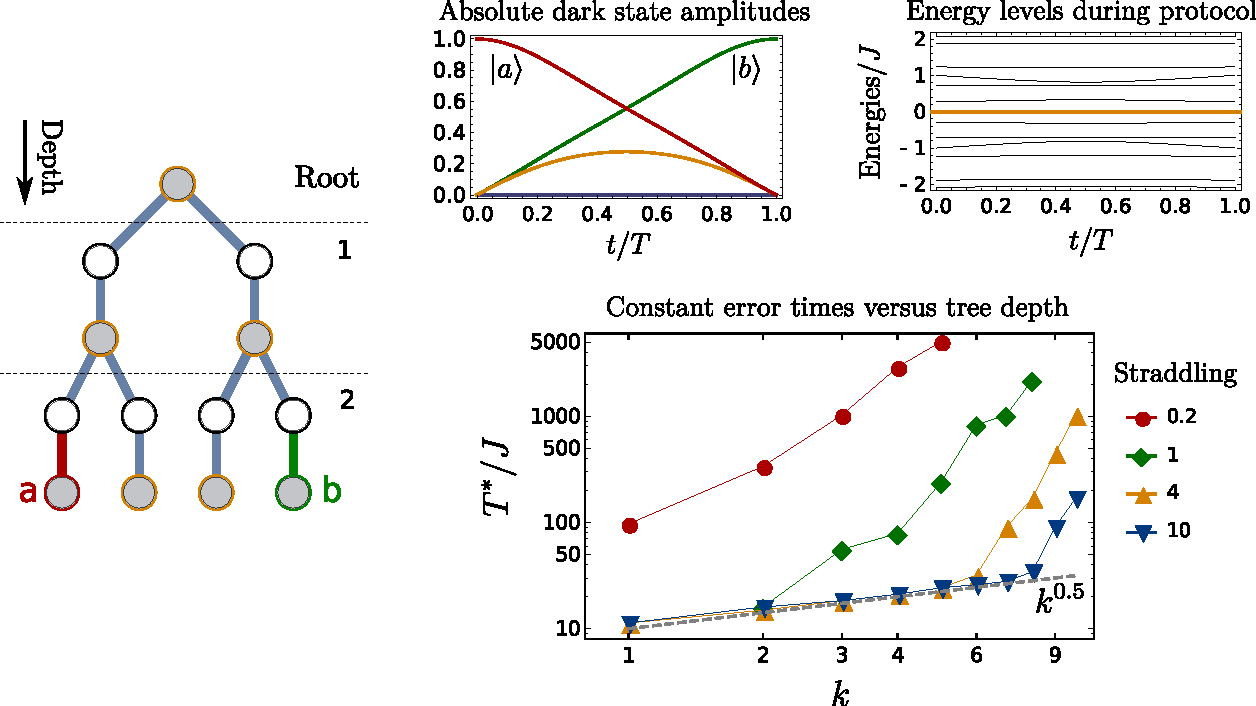
\includegraphics[width=\linewidth]{tree_scaling_horiz_2_thesis.pdf}
%
%
\caption{Simulation results on tree graphs are presented.  A tree of depth $k=2$ is shown on the left, with receivers $a$ and $b$ maximally separated. The top charts show the ideal state evolution over time, and the energy levels during the protocol. The bottom chart shows how the times $T^*$ required for constant fidelity increase steeply with $k$, except when sufficiently strong straddling is applied, leading to $T^*\propto k^{0.5}$ (dashed line). Note that the size of the graph is \emph{exponential} in $k$.}
\label{fig:tree}
\end{figure}

\paragraph{Transfer fidelities}
To assess the actual accuracy of our protocol, we numerically simulate the time evolution of a transfered state. As graphs, we choose subdivided binary trees of depth $k$, as these allow transfer between a large number of parties. For example, each leave (endpoint) of the tree is a potential party, allowing $|P| = 2^k$ different parties to participate. In our simulations, we choose to transfer a state between parties $a$ and $b$ which are at maximum distance from each other. This setup is depicted in \cref{fig:tree}. 

We define the transfer error as $\mathcal{E} = 1-| \bra{b} U_T \ket{a}|$, where $U_T$ denotes the unitary time-evolution operator as found by numerically solving Schr\"{o}dinger's Equation, and $T$ is the total protocol's time. We choose simple time-dependent couplings $f_a = J t/T$ and $f_b = J ( 1-t/T )$, while all other controls remain $f_v = 1$. Moreover, we define $T^*$ as the lowest time for which $\mathcal{E} < 0.05$, setting a bar for transfer with $95\%$ fidelity. 

Owing to the exponentially large size $|V|$ of the graphs, the time required rapidly increases with $k$ (\cref{fig:tree}). Interestingly, we find that the technique of straddling  \cite{Malinovsky1997,Greentree2004}, in which all controls $f_v$ except for $f_a$ and $f_b$ are multiplied by a factor $s$, flattens the scaling down to roughly $T^* \approx 10 \sqrt{k}$, up to a certain $k$ where the steep increase is observed again. Ref. \cite{Greentree2005} already predicted a favorable scaling $T^* \propto \sqrt{n}$ for linear chains of length $n$ in the strong straddling limit. It is surprising that here, we find a similar scaling in $k$ rather than $n$, even though the number of vertices increases exponentially in $k$.
 
There are various reasons to believe that the strong straddling scaling cannot remain valid for increasingly large systems, for example due to Lieb-Robinson bounds \cite{Lieb1972}. Still, with a modest straddling factor $s = 10$, transfer at favorable scaling $T^*\propto \sqrt{\log(|P|)}$ is observed for graphs of up to $1000$ sites, showing that near-term experiments can benefit from this effect. 



\section{Conclusion}
\label{sec:conclusion}
To summarize, we extend the set of graphs in which STIRAP-like protocols are known to work. The sufficient requirements are made precise in assumptions \emph{1} and \emph{2} of \cref{thm:transfer}, which can be guaranteed using the techniques in \cref{sec:viablegraphs}. We inherit the most important properties of the conventional protocols: the adiabatic controls do not require precise amplitudes or timings, the system's energy is \emph{exactly} zero at all times, and the fidelity is largely insensitive to decay on sites in $V_2$. Various extensions, such as straddling and multi-party transfer, can be readily incorporated. In the studied example of tree-shaped graphs, we find that with mild straddling the fidelities are much better than naively expected. 

As our requirements are sufficient but not necessary, we would be interested to see further work explore other graphs with unique zero eigenstates, and give guarantees on spectral gaps around the zero eigenvalue for specific graphs. Moreover, we look forward to seeing state-of-the-art experiments test our results in practice. 

